\documentclass[14pt]{extbook}
\usepackage{multicol, enumerate, enumitem, hyperref, color, soul, setspace, parskip, fancyhdr} %General Packages
\usepackage{amssymb, amsthm, amsmath, bbm, latexsym, units, mathtools} %Math Packages
\everymath{\displaystyle} %All math in Display Style
% Packages with additional options
\usepackage[headsep=0.5cm,headheight=12pt, left=1 in,right= 1 in,top= 1 in,bottom= 1 in]{geometry}
\usepackage[usenames,dvipsnames]{xcolor}
\usepackage{dashrule}  % Package to use the command below to create lines between items
\newcommand{\litem}[1]{\item#1\hspace*{-1cm}\rule{\textwidth}{0.4pt}}
\pagestyle{fancy}
\lhead{Progress Quiz 4}
\chead{}
\rhead{Version B}
\lfoot{8448-1521}
\cfoot{}
\rfoot{Fall 2020}
\begin{document}

\begin{enumerate}
\litem{
Find the equation of the line described below. Write the linear equation as $ y=mx+b $ and choose the intervals that contain $m$ and $b$.\[ \text{Perpendicular to } 7 x + 8 y = 10 \text{ and passing through the point } (2, -9). \]\begin{enumerate}[label=\Alph*.]
\item \( m \in [0.68, 1.09] \hspace*{3mm} b \in [-11.51, -11.03] \)
\item \( m \in [-1.64, -0.83] \hspace*{3mm} b \in [-6.99, -6.64] \)
\item \( m \in [1.06, 1.65] \hspace*{3mm} b \in [-11.51, -11.03] \)
\item \( m \in [1.06, 1.65] \hspace*{3mm} b \in [-11.09, -10.88] \)
\item \( m \in [1.06, 1.65] \hspace*{3mm} b \in [11.25, 11.54] \)

\end{enumerate} }
\litem{
Solve the linear equation below. Then, choose the interval that contains the solution.\[ \frac{8x -5}{3} - \frac{6x + 8}{7} = \frac{5x + 6}{6} \]\begin{enumerate}[label=\Alph*.]
\item \( x \in [3.7, 6.6] \)
\item \( x \in [1.2, 2] \)
\item \( x \in [16.2, 20.6] \)
\item \( x \in [-1.7, -0.6] \)
\item \( \text{There are no real solutions.} \)

\end{enumerate} }
\litem{
Write the equation of the line in the graph below in Standard form $Ax+By=C$. Then, choose the intervals that contain $A, B, \text{ and } C$.
\begin{center}
    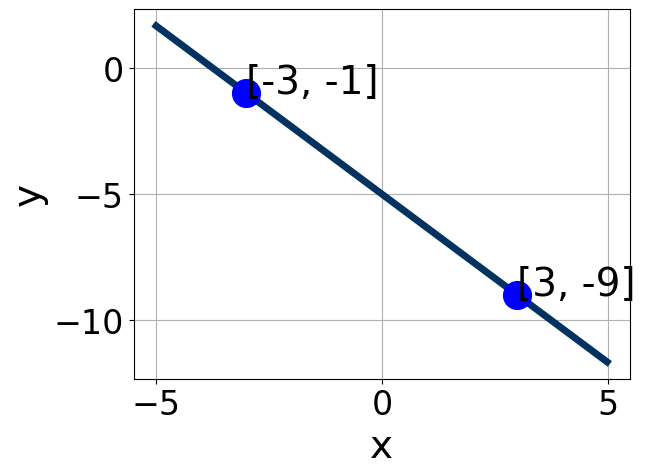
\includegraphics[width=0.5\textwidth]{../Figures/linearGraphToStandardB.png}
\end{center}
\begin{enumerate}[label=\Alph*.]
\item \( A \in [3, 10], \hspace{3mm} B \in [1.98, 3.41], \text{ and } \hspace{3mm} C \in [-15, -6] \)
\item \( A \in [-6, -1], \hspace{3mm} B \in [-4.04, -2.02], \text{ and } \hspace{3mm} C \in [12, 19] \)
\item \( A \in [0.33, 2.33], \hspace{3mm} B \in [-2.03, 0.5], \text{ and } \hspace{3mm} C \in [4, 6] \)
\item \( A \in [3, 10], \hspace{3mm} B \in [-4.04, -2.02], \text{ and } \hspace{3mm} C \in [12, 19] \)
\item \( A \in [0.33, 2.33], \hspace{3mm} B \in [0.82, 1.89], \text{ and } \hspace{3mm} C \in [-8, 1] \)

\end{enumerate} }
\litem{
Solve the linear equation below. Then, choose the interval that contains the solution.\[ \frac{-6x + 5}{7} - \frac{-6x -5}{6} = \frac{3x + 9}{2} \]\begin{enumerate}[label=\Alph*.]
\item \( x \in [0.4, 1.2] \)
\item \( x \in [-3.9, -2.3] \)
\item \( x \in [-1.4, -0.5] \)
\item \( x \in [-2.3, -1.6] \)
\item \( \text{There are no real solutions.} \)

\end{enumerate} }
\litem{
First, find the equation of the line containing the two points below. Then, write the equation as $ y=mx+b $ and choose the intervals that contain $m$ and $b$.\[ (4, -11) \text{ and } (5, -3) \]\begin{enumerate}[label=\Alph*.]
\item \( m \in [5, 9] \hspace*{3mm} b \in [43, 44] \)
\item \( m \in [-8, -5] \hspace*{3mm} b \in [37, 42] \)
\item \( m \in [5, 9] \hspace*{3mm} b \in [-9, -7] \)
\item \( m \in [5, 9] \hspace*{3mm} b \in [-15, -11] \)
\item \( m \in [5, 9] \hspace*{3mm} b \in [-45, -41] \)

\end{enumerate} }
\litem{
First, find the equation of the line containing the two points below. Then, write the equation as $ y=mx+b $ and choose the intervals that contain $m$ and $b$.\[ (5, 4) \text{ and } (-10, 6) \]\begin{enumerate}[label=\Alph*.]
\item \( m \in [-0.46, 0.01] \hspace*{3mm} b \in [-1.6, -0.7] \)
\item \( m \in [-0.46, 0.01] \hspace*{3mm} b \in [14.7, 17.3] \)
\item \( m \in [-0.02, 0.62] \hspace*{3mm} b \in [5, 10.6] \)
\item \( m \in [-0.46, 0.01] \hspace*{3mm} b \in [-6.1, -1.3] \)
\item \( m \in [-0.46, 0.01] \hspace*{3mm} b \in [2, 6.2] \)

\end{enumerate} }
\litem{
Find the equation of the line described below. Write the linear equation as $ y=mx+b $ and choose the intervals that contain $m$ and $b$.\[ \text{Perpendicular to } 3 x - 8 y = 10 \text{ and passing through the point } (9, -9). \]\begin{enumerate}[label=\Alph*.]
\item \( m \in [-3.3, -1.7] \hspace*{3mm} b \in [-23, -16] \)
\item \( m \in [-3.3, -1.7] \hspace*{3mm} b \in [12, 21] \)
\item \( m \in [0.5, 4.3] \hspace*{3mm} b \in [-33, -32] \)
\item \( m \in [-1.4, 2.5] \hspace*{3mm} b \in [12, 21] \)
\item \( m \in [-3.3, -1.7] \hspace*{3mm} b \in [-16, -12] \)

\end{enumerate} }
\litem{
Write the equation of the line in the graph below in Standard form $Ax+By=C$. Then, choose the intervals that contain $A, B, \text{ and } C$.
\begin{center}
    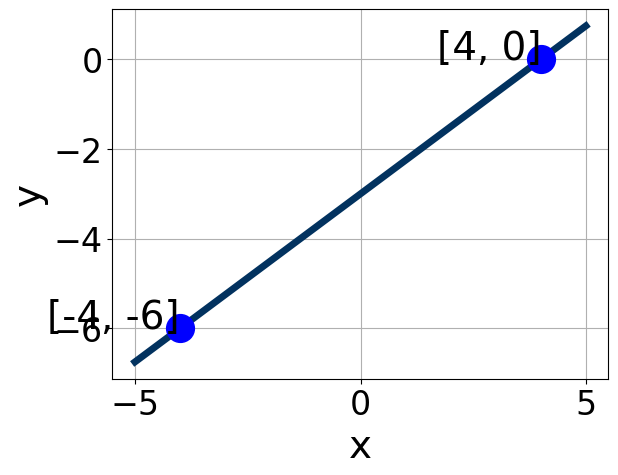
\includegraphics[width=0.5\textwidth]{../Figures/linearGraphToStandardCopyB.png}
\end{center}
\begin{enumerate}[label=\Alph*.]
\item \( A \in [3, 5], \hspace{3mm} B \in [2.03, 4.19], \text{ and } \hspace{3mm} C \in [5, 17] \)
\item \( A \in [-5, -1], \hspace{3mm} B \in [2.03, 4.19], \text{ and } \hspace{3mm} C \in [5, 17] \)
\item \( A \in [-0.75, 0.25], \hspace{3mm} B \in [0.33, 3.14], \text{ and } \hspace{3mm} C \in [2, 8] \)
\item \( A \in [-0.75, 0.25], \hspace{3mm} B \in [-1.05, -0.45], \text{ and } \hspace{3mm} C \in [-3, -1] \)
\item \( A \in [3, 5], \hspace{3mm} B \in [-5.68, -3.67], \text{ and } \hspace{3mm} C \in [-16, -8] \)

\end{enumerate} }
\litem{
Solve the equation below. Then, choose the interval that contains the solution.\[ -7(-19x + 8) = -9(10x + 17) \]\begin{enumerate}[label=\Alph*.]
\item \( x \in [0.38, 1.04] \)
\item \( x \in [-1.43, -0.44] \)
\item \( x \in [-0.57, 0.08] \)
\item \( x \in [4.67, 5.95] \)
\item \( \text{There are no real solutions.} \)

\end{enumerate} }
\litem{
Solve the equation below. Then, choose the interval that contains the solution.\[ -14(18x -2) = -12(-5x -13) \]\begin{enumerate}[label=\Alph*.]
\item \( x \in [0.84, 1.05] \)
\item \( x \in [-0.54, -0.31] \)
\item \( x \in [-0.6, -0.54] \)
\item \( x \in [0.47, 0.68] \)
\item \( \text{There are no real solutions.} \)

\end{enumerate} }
\end{enumerate}

\end{document}